In the past years, the study of the VBS processes has attracted lots of interests in the theory community, (see \emph{e.g.}\ Ref.~\cite{Rauch:2016pai}).
The activities range from providing precise predictions for the VBS signal and background processes in the Standard Model, to studying the sensitivity of these 
processes on new physics effects, by mean of effective theories or by studying the polarisation patterns of the heavy gauge bosons involved.
The program of the meeting reflects these avenues.

\subsection{Complete NLO corrections to ${\rm W^+ W^+}$ scattering - M. Pellen}

The first VBS process that has been observed during the run~I of the LHC is the same-sign WW production~\cite{Aad:2014zda,Aaboud:2016ffv,Khachatryan:2014sta}.
This observation has already been confirmed by a measurement of the CMS collaboration at the 13 TeV run~II~\cite{CMS:2017adb}.
In view of the growing mole of data which will be collected by the experiments, and of the consequent reduction of the uncertainties affecting these measurements, precise theoretical predictions become necessary.

In that respect next-to-leading order (NLO) QCD and electroweak (EW) corrections to such signatures should be computed.
So far, NLO computations have focused on NLO QCD corrections to the VBS process~\cite{Jager:2009xx,Jager:2011ms,Denner:2012dz,Rauch:2016pai} and its QCD-induced irreducible background process~\cite{Melia:2010bm,Melia:2011gk,Campanario:2013gea,Baglio:2014uba,Rauch:2016pai}.
No NLO EW corrections have been computed and the NLO QCD computations relied on the so-called VBS approximation.
In Refs.~\cite{Biedermann:2016yds,Biedermann:2017bss}, for the first time, all leading order (LO) and NLO contributions to the full ${\rm p}{\rm p}\to\mu^+\nu_\mu{\rm e}^+\nu_{\rm e}{\rm j}{\rm j}$ process have been reported.
As the full amplitudes are used, this amounts to compute three LO contributions and four NLO contributions.
At LO, the three contributions are the EW process (order $\mathcal{O}{\left(\alpha^{6}\right)}$), its QCD-induced counterpart (order $\mathcal{O}{\left(\alpha_{\rm s}\alpha^{5}\right)}$) as well as the interference (order $\mathcal{O}{\left(\alpha_{\rm s}^2\alpha^{4}\right)}$).
Due to the VBS event selection applied to the final state, the full process is dominated by the purely EW contribution (see Table~\ref{table:LOVBS}).
This EW contribution feature the VBS diagrams but also background diagrams where for example the W bosons are simply radiated off the quark lines.

\begin{table}
\begin{center}
\begin{tabular}{|l||c|c|c||c|}
\hline
Order & $\mathcal{O}{\left(\alpha^{6}\right)}$ & $\mathcal{O}{\left(\alpha_{\rm s}\alpha^{5}\right)}$ & $\mathcal{O}{\left(\alpha_{\rm s}^2\alpha^{4}\right)}$ & Sum \\
\hline
\hline
${\sigma_{\mathrm{LO}}}$ [fb] 
& $1.4178(2)$
& $0.04815(2)$
& $0.17229(5)$
& $1.6383(2)$ \\
\hline
\end{tabular}
\end{center}
\caption{
Fiducial cross section from Ref.~\cite{Biedermann:2017bss} at LO for the process ${\rm p}{\rm p}\to\mu^+\nu_\mu{\rm e}^+\nu_{\rm e}{\rm j}{\rm j}$, at
orders  $\mathcal{O}{\left(\alpha^{6}\right)}$, $\mathcal{O}{\left(\alpha_{\rm s}\alpha^{5}\right)}$, and $\mathcal{O}{\left(\alpha_{\rm s}^2\alpha^{4}\right)}$.
The sum of all the LO contributions is in the last column and all contributions expressed in femtobarn. 
The statistical uncertainty from the Monte Carlo integration on the last digit is given in parenthesis.}
\label{table:LOVBS}
\end{table}

At NLO, the four contributions arise at the orders $\mathcal{O}{\left(\alpha^{7}\right)}$, $\mathcal{O}{\left(\alpha_{\rm s}\alpha^{6}\right)}$, $\mathcal{O}{\left(\alpha_{\rm s}^{2}\alpha^{5}\right)}$, and $\mathcal{O}{\left(\alpha_{\rm s}^{3}\alpha^{4}\right)}$. 
An interesting feature is that the orders $\mathcal{O}{\left(\alpha_{\rm s}\alpha^{6}\right)}$ and $\mathcal{O}{\left(\alpha_{\rm s}^{2}\alpha^{5}\right)}$ receive both EW and QCD corrections.
Thus, at NLO (as opposed to LO) it is not possible to strictly distinguish the EW process from the QCD-induced process.
As it can be seen from Table~\ref{table:NLOVBS}, at the level of the fiducial cross section, the largest corrections are the one of order $\mathcal{O}{\left(\alpha^{7}\right)}$.
These are the NLO EW corrections to the EW processes.

\begin{table}
\begin{center}
\begin{tabular}{|l||c|c|c|c||c|}
\hline
Order & $\mathcal{O}{\left(\alpha^{7}\right)}$ & $\mathcal{O}{\left(\alpha_{\rm s}\alpha^{6}\right)}$ & $\mathcal{O}{\left(\alpha_{\rm s}^{2}\alpha^{5}\right)}$ & $\mathcal{O}{\left(\alpha_{\rm s}^{3}\alpha^{4}\right)}$ & Sum \\
\hline
\hline 
${\delta \sigma_{\mathrm{NLO}}}$ [fb] 
& $-0.2169(3)$ 
& $-0.0568(5)$
& $-0.00032(13)$
& $-0.0063(4)$ 
& $-0.2804(7)$ \\
\hline
$\delta \sigma_{\mathrm{NLO}}/\sigma_{\rm LO}$ [\%] & $-13.2$ & $-3.5$ & $0.0$ & $-0.4$ & $-17.1$ \\
\hline
\end{tabular}
\end{center}
\caption{
NLO corrections from Ref.~\cite{Biedermann:2017bss} for the process ${\rm p}{\rm p}\to\mu^+\nu_\mu{\rm e}^+\nu_{\rm e}{\rm j}{\rm j}$ at the orders 
$\mathcal{O}{\left(\alpha^{7}\right)}$, $\mathcal{O}{\left(\alpha_{\rm s}\alpha^{6}\right)}$, $\mathcal{O}{\left(\alpha_{\rm s}^{2}\alpha^{5}\right)}$, and $\mathcal{O}{\left(\alpha_{\rm s}^{3}\alpha^{4}\right)}$.
The sum of all the NLO contributions is in the last column.
The contribution $\delta\sigma_{\mathrm{NLO}}$ corresponds to the absolute correction while $\delta \sigma_{\mathrm{NLO}}/\sigma_{\rm LO}$ gives the relative correction normalised to the sum of all LO contributions.
The absolute contributions are expressed in femtobarn while the relative ones are expressed in per cent.
The statistical uncertainty from the Monte Carlo integration on the last digit is given in parenthesis.}
\label{table:NLOVBS}
\end{table}

This is also reflected in two differential distributions in the the transverse momentum for the hardest jet and invariant mass for the two leading jets in Fig.~\ref{fig:VBSALL}.
% Each contribution (both LO and NLO) shows distinctive features.
At LO, the QCD induced process as well as the interference are rather suppressed due to the typical VBS event selection (as for the fiducial cross section).
This is exemplified in the invariant mass of the two leading jet where at high invariant mass, the QCD-induced background becomes negligible.
At NLO, the bulk of the corrections originate from the large EW to the EW process at order $\mathcal{O}{\left(\alpha^{7}\right)}$.
In particular, they display the typical behaviour of Sudakov logarithms that grow large in the high energy limit.
Note that the contribution from initial state photon is also shown but is not taken into account in the definition of the NLO predictions.
This contribution is rather small and relatively constant in shape over the whole range studied here.
Finally, as at NLO it is not possible to isolate the EW production from its irreducible backgrounds, a global measurement of the full process ${\rm p}{\rm p}\to\mu^+\nu_\mu{\rm e}^+\nu_{\rm e}{\rm j}{\rm j}$ with all components is desirable.
% Hence in Fig.~\ref{fig:VBSAAL_sum}, the sum all the contributions at both LO and NLO is shown in a combined prediction.

\begin{figure}
% \hspace{-2cm}
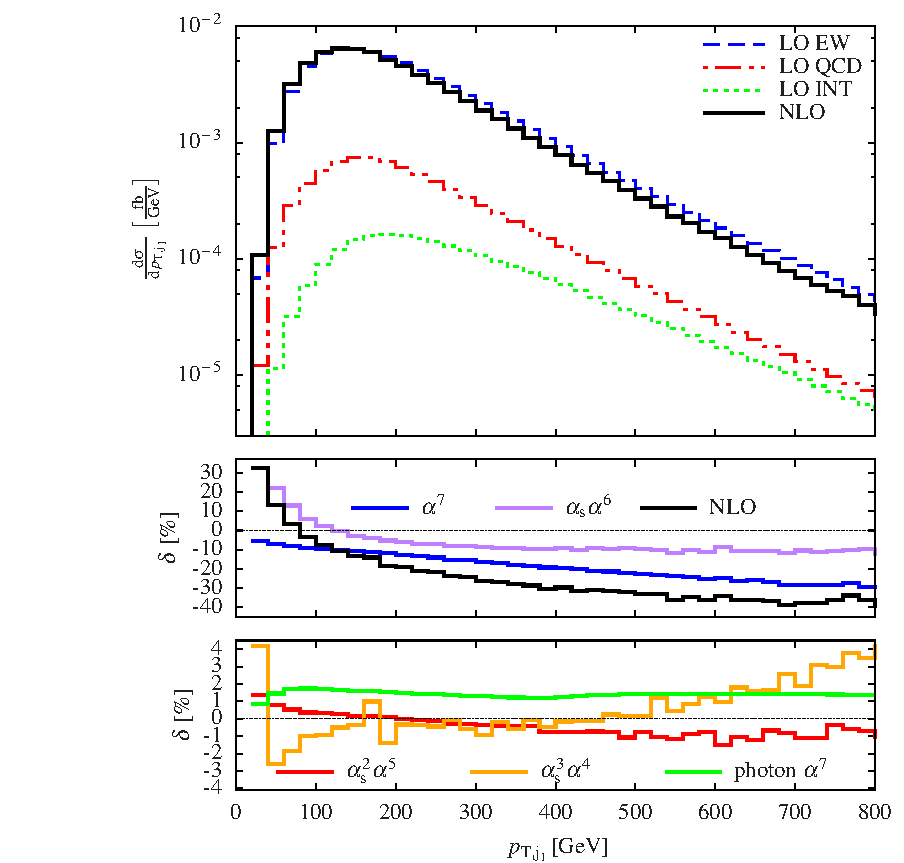
\includegraphics[width=.47\textwidth]{WG1_plots/histogram_transverse_momentum_j1}
\hfill
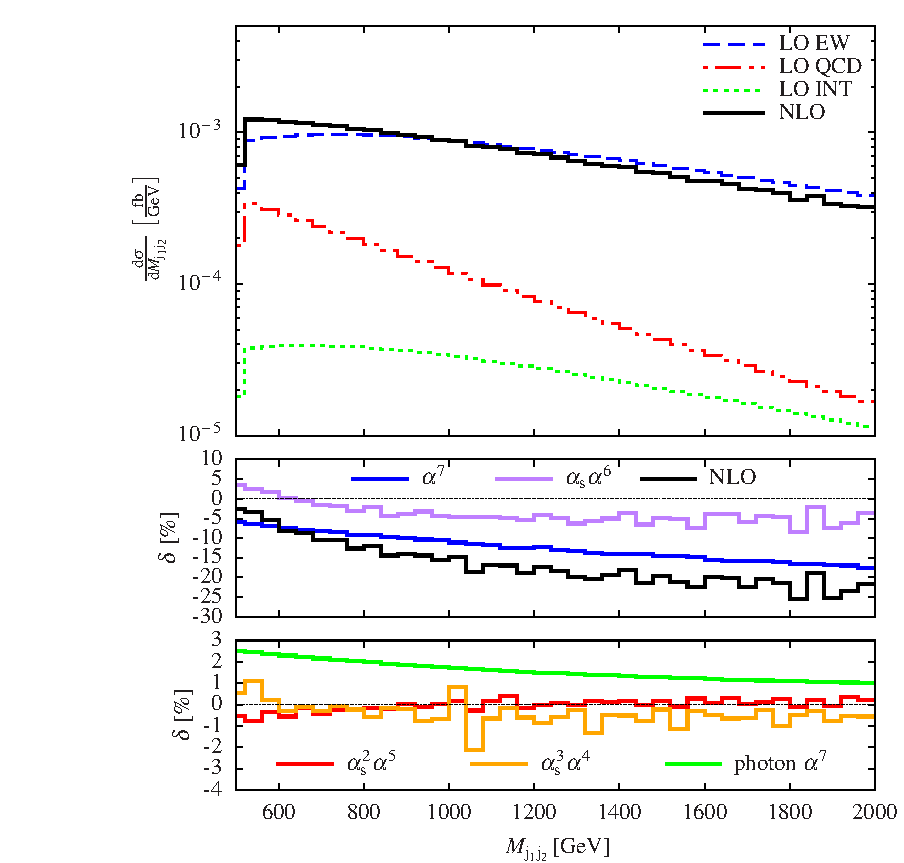
\includegraphics[width=.47\textwidth]{WG1_plots/histogram_invariant_mass_mjj12}
% \vspace*{-1em}
\caption{Differential distributions from Ref.~\cite{Biedermann:2017bss} for ${\rm p}{\rm p}\to\mu^+\nu_\mu{\rm e}^+\nu_{\rm e}{\rm j}{\rm j}$:
transverse momentum for the hardest jet~(left) and invariant mass for the two leading jets~(right).
The two lower panels show the relative NLO corrections with respect to the full LO in per cent,
defined as $\delta_i = \delta \sigma_{i} / \sum \sigma_{\text{LO}}$, 
where $i=\mathcal{O}{\left(\alpha^{7}\right)},\mathcal{O}{\left(\alpha_{\rm s}\alpha^{6}\right)},\mathcal{O}{\left(\alpha_{\rm s}^2\alpha^{5}\right)},\mathcal{O}{\left(\alpha_{\rm s}^3\alpha^{4}\right)}$.
In addition, the NLO photon-induced contributions of order $\mathcal{O}{\left(\alpha^{7}\right)}$ is provided separately.}
\label{fig:VBSALL}
\end{figure}

% \begin{figure}
% % \hspace{-2cm}
% 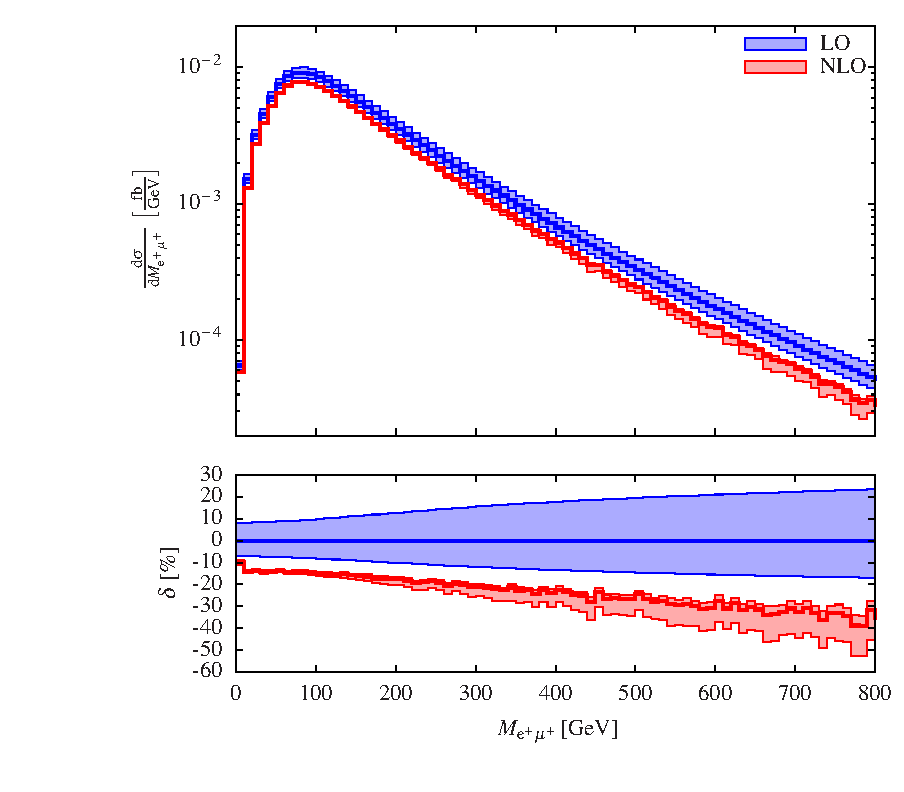
\includegraphics[width=.47\textwidth]{WG1_plots/histogram_invariant_mass_epmu_scale}
% \hfill
% 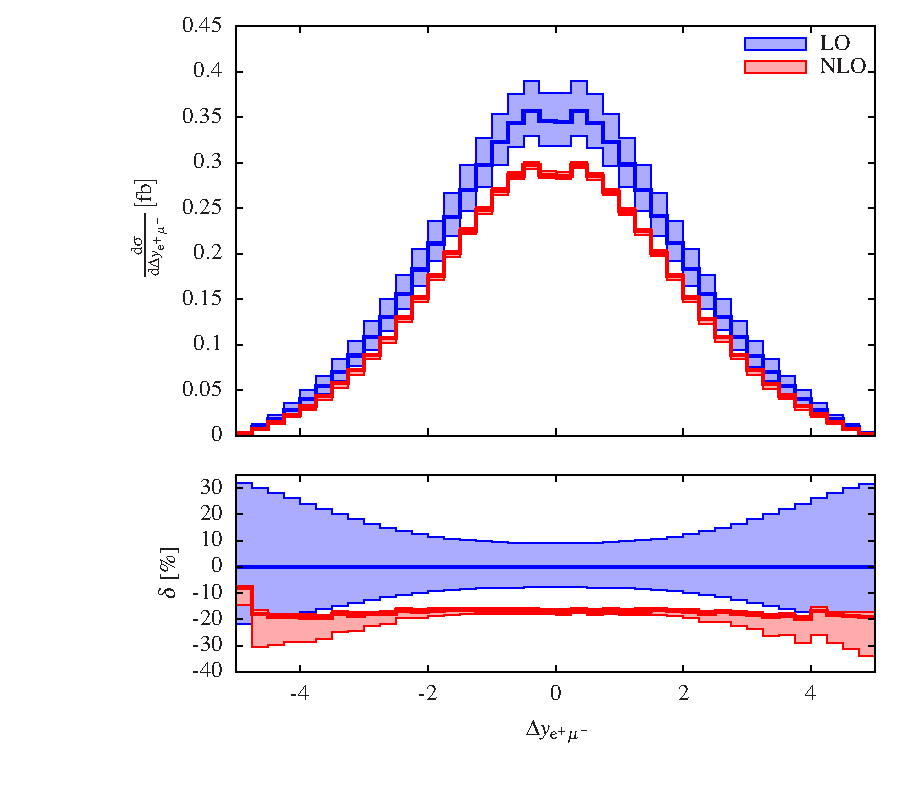
\includegraphics[width=.47\textwidth]{WG1_plots/histogram_rapidity_separation_pomu_scale}
% % \vspace*{-1em}
% \caption{Differential distributions from Ref.~\cite{Biedermann:2017bss} for ${\rm p}{\rm p}\to\mu^+\nu_\mu{\rm e}^+\nu_{\rm e}{\rm j}{\rm j}$:
% invariant mass of the positron and anti-muon system~(left) and rapidity separation between the electron and anti-muon~(right).
% The upper panels show the sum of all LO and NLO contributions with scale variation.
% The lower panels show the relative corrections in per cent.}
% \label{fig:VBSAAL_sum}
% \end{figure}

As shown previously, the EW corrections of order $\mathcal{O}\left(\alpha^7\right)$ are the dominant NLO contributions.
These originate from Sudakov logarithms that grow negatively large in the high energy limit.
This is shown in the differential distribution in the transverse momentum of the hardest jet on the left hand-side of Fig.~\ref{fig:VBSEW}.
Usually these EW corrections are particularly large only in phase space regions which are suppressed.
Hence the impact at the level of the total fiducial cross section is usually rather limited.
This is not the case here where the corrections are already large at the level of the cross section and reach $-16\%$ \cite{Biedermann:2016yds}.
The origin of these large EW corrections are virtual corrections and in particular the ones corresponding to the insertion of massive particles in the scattering process \cite{Biedermann:2016yds}.
Hence, large NLO EW corrections are an intrinsic feature of VBS at the LHC.
As the EW corrections are particularly large, it might be possible to measure them at a high luminosity LHC, hence probing the EW sector of the Standard Model to very high precision.
This is illustrated on the left hand-side of Fig.~\ref{fig:VBSEW} where the band represent the estimated statistical error for a high-luminosity LHC collecting $3000{\rm fb}^{-1}$.

\begin{figure}
% \hspace{-2cm}
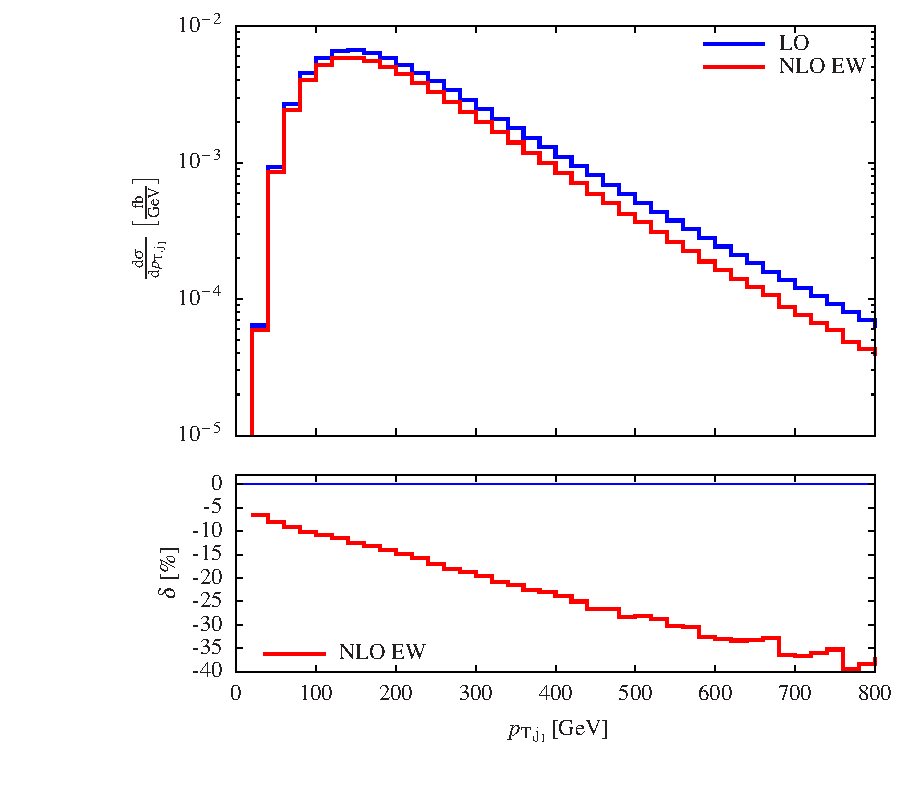
\includegraphics[width=.47\textwidth]{WG1_plots/histogram_transverse_momentum_j1_ew}
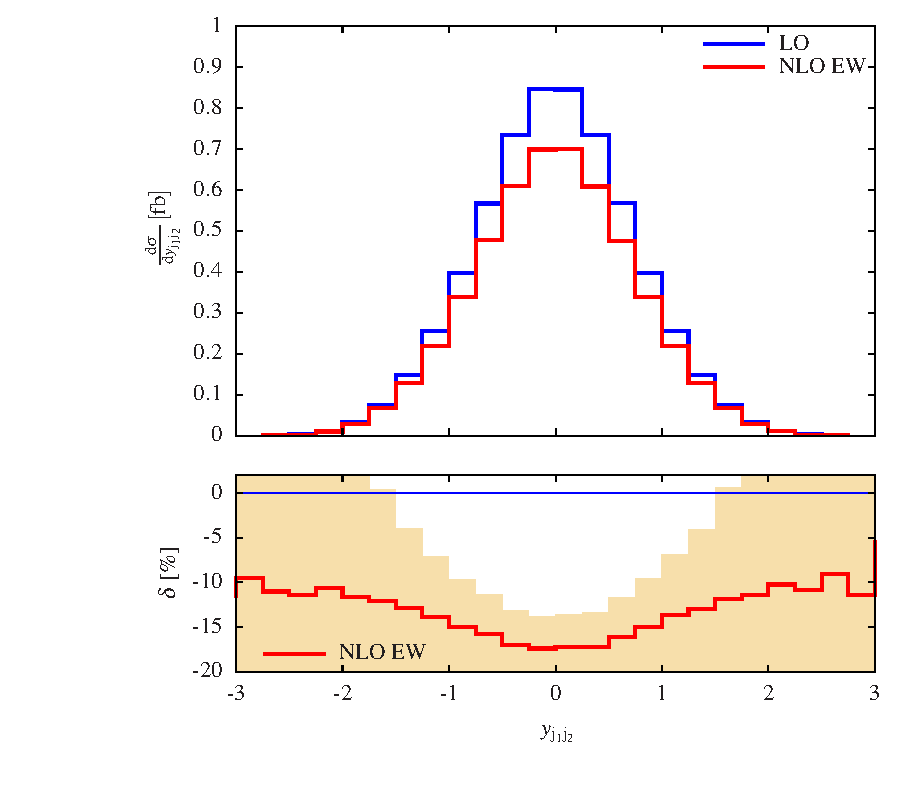
\includegraphics[width=.47\textwidth]{WG1_plots/histogram_rapidity_j1j2_ew}
% \vspace*{-1em}
\caption{Differential distributions from Ref.~\cite{Biedermann:2016yds} for ${\rm p}{\rm p}\to\mu^+\nu_\mu{\rm e}^+\nu_{\rm e}{\rm j}{\rm j}$ including NLO EW corrections (upper panel) and relative NLO EW corrections (lower panel).
Left plot: Invariant-mass distribution of the four leptons.
Right plot: Rapidity distribution of the leading jet pair.
The yellow band describes the expected statistical experimental uncertainty for a high-luminosity LHC collecting $3000{\rm fb}^{-1}$ and represents a relative variation of $\pm 1/\sqrt{N_{\rm obs}}$ where $N_{\rm obs}$ is the number of observed events in each bin.}
\label{fig:VBSEW}
\end{figure}

\subsection{Monte Carlo comparisons for ${\rm W^+ W^+}$ scattering - M. Zaro}
In the last decade many codes capable of performing VBS simulations have appeared.
Within a network such as VBSCan it is therefore natural to perform 
a quantitative comparison of these codes, both to cross-validate the results and to assess the impact of the different approximations which are used.
In fact, already at LO, when considering the process ${\rm p}{\rm p}\to\mu^+\nu_\mu{\rm e}^+\nu_{\rm e}{\rm j}{\rm j}$ at order $\mathcal O (\alpha^6)$, the various implementations VBS simulations are different.
They differ, for example
by the (non-)inclusion of diagrams with vector bosons in the $s$-channel or by the treatment of interferences between diagrams.
The reason of these differences is that, 
when typical signal cuts for VBS are imposed, these effects turn to be small on rates and distributions.

In our comparison, we use the following codes: {\bf ADD/CHECK CITES} 
{\sc Bonsay}~\cite{},
{\sc MadGraph5\_aMC@NLO}~\cite{Alwall:2014hca}, 
{\sc Powheg}~\cite{},

The program {\sc Recola+MoCaNLO} is made of a flexible Monte Carlo program dubbed {\sc MoCaNLO}~\cite{MoCaNLO} and the general matrix element generator {\sc Recola} \cite{Actis:2012qn,Actis:2016mpe}.
To numerically evaluate the one-loop scalar and tensor integrals, {\sc Recola} relies on the {\sc Collier} library \cite{Denner:2014gla,Denner:2016kdg},
These tools have been successfully used for the computation of NLO corrections for VBS~\cite{Biedermann:2016yds,Biedermann:2017bss}.

{\sc VBFNLO}~\cite{Arnold:2008rz, Arnold:2011wj, Baglio:2014uba} is a flexible
parton-level Monte Carlo for processes with electroweak bosons. It
allows the calculation of VBS processes at NLO QCD in the VBF
approximation and including the s-channel triboson contribution,
neglecting interferences between the two. Besides the SM, also anomalous
couplings of the Higgs and gauge bosons can be simulated.

{\sc Whizard}~\cite{Moretti:2001zz,Kilian:2007gr}.\\
DESCRIPTION OF CODES\\
The complete comparison of the codes will be published in a separate work. Here, we present some preliminary results obtained at LO ($\mathcal O (\alpha^6)$) and including
NLO QCD corrections at fixed-order $\mathcal O (\alpha^6\alpha_s)$, for the process ${\rm p}{\rm p}\to\mu^+\nu_\mu{\rm e}^+\nu_{\rm e}{\rm j}{\rm j}$.
In Tab.~\ref{tab:wg1_codes} the details of the various codes are reported. In particular, it is specified whether
\begin{itemize}
    \item all $s-$ and $t/u-$channel diagrams that lead to the considered final state are included;
    \item interferences between diagrams are included at LO;
    \item diagrams which do not feature two resonant vector bosons are included;
    \item the so-called non-factorizable (NF) QCD corrections, that is the corrections where (real or virtual) gluons are exchanged between different quark lines,
        are included;
    \item EW corrections to the $\mathcal O (\alpha^5\alpha_s)$ interference are included. These corrections are of the same order as the NLO QCD corrections to
        the  $\mathcal O (\alpha^6$) term.
\end{itemize}
%
\begin{table}
    \footnotesize
    \begin{tabularx}{\textwidth}{c|c|X|X|X|X|X}
        Contact person  &  Code  &  $\mathcal O(\alpha^6)$ $|s|^2/$ $|t|^2/|u|^2$  &  $\mathcal O(\alpha^6)$ interf.  &  Non-res.  &  NF QCD  &  EW corr. to $\mathcal O(\alpha^5\alpha_s)$  \\
        \hline
        \hline
        A. Karlberg  &  {\sc POWHEG}  &  $t/u$  &  No  &  Yes  &  No  &  No  \\
        M. Pellen    &  {\sc Recola}  &  Yes  &  Yes  &  Yes  &  Yes  &  Yes  \\
        M. Rauch     &  {\sc VBFNLO}  &  Yes  &  No  &  Yes  &  No  &  No  \\
        C. Schwan    &  {\sc BONSAY}  &  $t/u$  &  No  &  Yes, virt. No  &  No  &  No  \\
        M. Zaro      &  {\sc MG5\_aMC}  &  Yes  &  Yes  &  No virt.  &  No  &  No \\
        J. Reuter    &  {\sc Whizard}  &    &    &    &    &  
    \end{tabularx}
    \caption{\label{tab:wg1_codes} Summary of the different properties of the codes employed in the comparison.}
\end{table}
%

We simulate VBS production at the LHC, with a center-of-mass energy $\sqrt s = 13 \TeV$. We assume five massless flavours in the proton, and employ the NNPDF~3.0 parton 
density~\cite{Ball:2014uwa}
with NLO QCD evolution (the {\tt lhaid} in LHAPDF6~\cite{Buckley:2014ana} for this set is 260000) and strong coupling constant $\alpha_s\left( \MZ \right) = 0.118$. Since
the employed PDF set has no photonic density, photon-induced processes are not considered. Initial-state collinear singularity are factorised with the  ${\overline{\rm MS}}$ 
scheme, consistently with what is done in NNPDF.\\
We use the following values for the mass and width of the massive particles:
% 
\begin{alignat}{2}
                  \Mt   &=  173.21\GeV,       & \quad \quad \quad \Gt &= 0 \GeV,  \nonumber \\
                \MZOS &=  91.1876\GeV,      & \quad \quad \quad \GZOS &= 2.4952\GeV,  \nonumber \\
                \MWOS &=  80.385\GeV,       & \GWOS &= 2.085\GeV,  \nonumber \\
                M_{\rm H} &=  125.0\GeV,       &  \GH   &=  4.07 \times 10^{-3}\GeV,
\end{alignat}
and renormalise the EW coupling in the $G_\mu$ scheme \cite{Denner:2000bj} where
\begin{equation}
    G_{\mu}    = 1.16637\times 10^{-5}\GeV.
\end{equation}
The derived value of the EW coupling $\alpha$, corresponding to our choice of input parameters, is 
\begin{equation}
 \alpha = 7.555310522369 \times 10^{-3}. \\
\end{equation}
We employ the complex-mass scheme~\cite{} to treat unstable intermediate particles in a gauge-invariant manner {\bf CHECK THAT ALL CODES USE THE CMS}.\\

Cross sections and distribution are computed within the following VBS cuts inspired from experimental measurements \cite{Aad:2014zda,Aaboud:2016ffv,Khachatryan:2014sta,CMS:2017adb}: 
\begin{itemize}
    \item The two same-sign charged leptons are required to have
        \begin{align}
         \ptsub{\Pl} >  20\GeV,\qquad |y_{\Pl}| < 2.5, \qquad \Delta R_{\Pl\Pl}> 0.3\,.
        \end{align}
    \item The total missing transverse energy, computed from the vectorial sum of the transverse momenta of the two neutrinos in the event,
        is required to be
        \begin{align}
          \etsub{\text{miss}}=p_{\rm T, miss} >  40\GeV\,.
        \end{align}
    \item QCD partons (quark and gluons) are clustered together using the anti-$k_T$ algorithm~\cite{} with distance parameter $R=0.4$. Jets are required
        to have
        \begin{align}
         \ptsub{\Pj} >  30\GeV, \qquad |y_\Pj| < 4.5, \qquad \Delta R_{\Pj\Pl} > 0.3 \,.
        \end{align}
        On the two jets with largest transverse-momentum the following invariant-mass and rapidity-separation cuts are imposed
        \begin{align}
         m_{\Pj \Pj} >  500\GeV,\qquad |\Delta y_{\Pj \Pj}| > 2.5.
        \end{align}
%         Finally, all jest in the event are required to be separated from charged leptons:
%         \begin{align}
%          \qquad\Delta R_{\Pj\Pl} > 0.3 .
%         \end{align}
    \item When EW corrections are computed, real photons and charged fermion are clustered together using the anti-$k_T$ algorithm with 
        radius parameter $R=0.1$. In this case, leptons and quarks mentioned above must be understood as {\it dressed fermions}. Photons
        which are not combined at this step are clustered with QCD partons to form jets as it is described previously.
\end{itemize}

In Tab.~\ref{tab:wg1_LOrates} we report the total rates at LO accuracy obtained with the set-up described above, and in Fig.~\ref{fig:wg1_mjj-llLO} we show the results
for the tagging-jet (left) and lepton-pair (right) invariant-mass distribution. In both cases we see an excellent agreement among the various tools, which confirms the fact
that contributions from $s-$channel diagrams as well as from non-resonant configurations are strongly suppressed in the fiducial region.
\begin{table}[h!]
    \centering
    \begin{tabular}{c|c}
        Code  &  $\sigma[\rm{fb}]$  \\
        \hline
        \hline
        {\sc POWHEG}  &  $1.5573 \pm 0.0003$ \\
        {\sc Recola}\+{\sc MoCaNLO}  &  $1.5503 \pm 0.0003$ \\
        {\sc VBFNLO}  &  $1.5538 \pm 0.0002$ \\
        {\sc BONSAY}  &  $1.5524 \pm 0.0002$ \\
        {\sc MG5\_aMC}&  $1.547 \pm 0.001$  \\ 
        {\sc Whizard}&  $ 1.5539 \pm 0.0004 $   
    \end{tabular}
    \caption{\label{tab:wg1_LOrates} LO rates within VBS cuts from the different codes.}
\end{table}
%
\begin{figure}[h!]
   \centering
   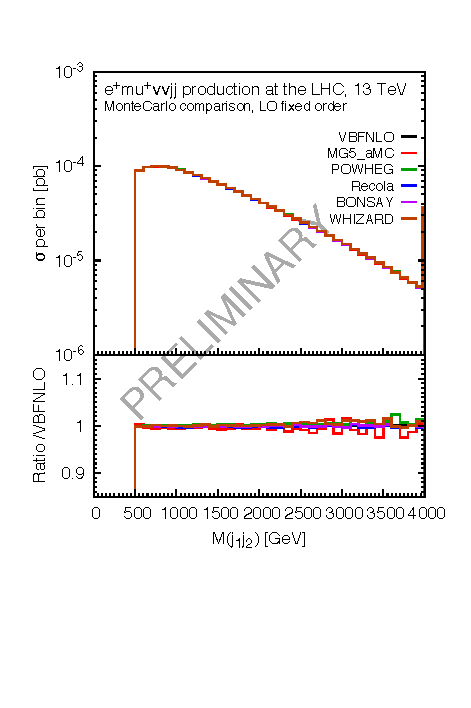
\includegraphics[width=0.49\textwidth,angle=0,clip=true,trim={0.4cm 2.5cm 0.6cm 1.cm}]{figures/mjj_LO.pdf}
   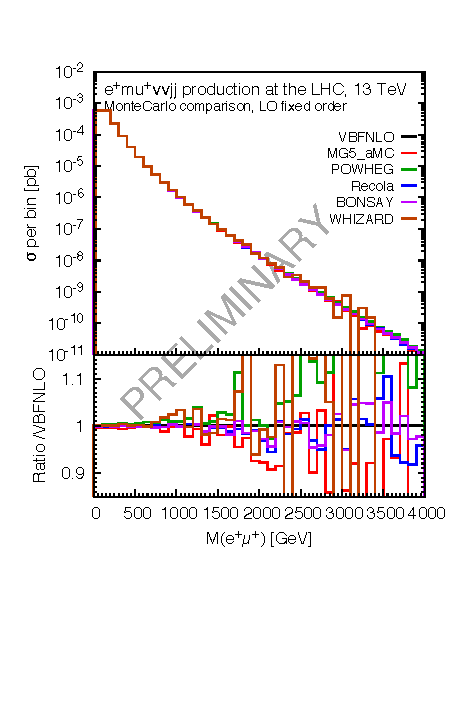
\includegraphics[width=0.49\textwidth,angle=0,clip=true,trim={0.4cm 2.5cm 0.6cm 1.cm}]{figures/mll_LO.pdf}
\caption{\label{fig:wg1_mjj-llLO}Invariant-mass of the two tagging jets (left) and of the two leptons (right), at LO.
}
\end{figure}
%
\begin{table}[h!]
    \centering
    \begin{tabular}{c|c|c|c}
        Code  &  $\sigma[\rm{fb}]$  &  $\sigma(n_j=2)[\rm{fb}]$  &  $\sigma(n_j=3)[\rm{fb}]$\\
        \hline
        \hline
        {\sc POWHEG}  &  $1.334 \pm 0.0003$  &  $0.808 \pm  0.001$  &  $0.5260 \pm 0.0005$\\
        {\sc Recola}\+{\sc MoCaNLO}  &  $1.317 \pm 0.004 $ \\
        {\sc VBFNLO}  &  $1.3531 \pm 0.0003$  &  $0.8264 \pm  0.0003$  &  $0.5267 \pm 0.0001$\\
        {\sc BONSAY}  &  $1.3366 \pm 0.0009$  &  $0.8199 \pm  0.0008$  &  $0.51663 \pm 0.00007$ \\
        {\sc MG5\_aMC}&  $1.318  \pm 0.003$  &  $0.781 \pm  0.004$  &  $0.5374 \pm 0.0016$\\
    \end{tabular}
    \caption{\label{tab:wg1_NLOrates} NLO rates within VBS cuts from the different codes. {\bf keep or drop jet rates?}}
\end{table}
At NLO, rates show slightly larger discrepancies, as it can be observed in Tab.~\ref{tab:wg1_NLOrates}. This is most likely due to low dijet invariant-mass configurations, where
$s-$channel diagrams and interferences are less suppressed than at LO, because of the presence of extra QCD radiation.

We conclude this section by recalling that the results presented must be regarded as preliminary.
In the coming months, this work will be enlarged to include comparison of predictions at NLO QCD matched to parton shower or with EW corrections, 
as well as to study the effect of changing 
the VBS cuts. The QCD-induced background will also be studied.

\subsection{Polarisation of vector bosons - E. Maina}

New physics model could lead to large contributions to the longitudinal polarisation of heavy gauge bosons [citation?].
Hence it is of prime importance to study the polarisation of the heavy gauge bosons and their effects both in the Standard Model and beyond.
In particular, it is very important to devise methods that allow for such studies.
Thus, a starting point is to establish these methods first for the Standard Model.
In this respect, a new method has been proposed and applied to the scattering of two W bosons of opposite charge.

First, a matrix element squared can be written in general as

\begin{equation}
\label{eq:polarisation}
 \mathcal{A}^2 = \sum_{\lambda} \mathcal{A}^2_{\lambda, \lambda} + \sum_{\lambda \neq \lambda'} \mathcal{A}^2_{\lambda, \lambda'}, 
\end{equation}
%
where $\lambda$ and $\lambda'$ represent the polarisations of the heavy gauge bosons.
Usually the last term of Eq.~\eqref{eq:polarisation} is assumed to be zero.
But this is only true when ones integrates over the full phase space over the variable $\phi$.
In experiments, it is never the case as experimental measurements are never done fully inclusively.
Indeed they always include event selections that cut into the phase space and make the use of a full computation necessary.

Second, an amplitude can be formally divided into resonant and non-resonant contributions as

\begin{equation}
\mathcal{A} = \mathcal{A}_{\rm res} + \mathcal{A}_{\rm non-res} .
\end{equation}
%
Non-resonant propagators cannot be interpreted as W production.
Hence, one should only retain the resonant part of the process.
To achieve this in a gauge invariant way, one can use the double-pole approximation where only diagrams featuring two W-boson propagators are selected.
This sub-set of diagrams is then evaluated with an on-shell kinematic.
But on-shell kinematics are not unique so one should use an on-shell projection that should fulfil the following criteria:
[To be added]
In such a way, one can set a given polarisation to the W bosons in a gauge invariant manner.

In order to be able to integrate fully over the variable $\phi$, one should consider a typical VBS event selection but without any cuts on the final state leptons.
If one consider a polarised ${\rm W^-}$-boson and a non-polarised ${\rm W^-}$ boson, one observes that the effect of the interferences between different polarisations (second term of Eq.~\eqref{eq:polarisation}) is below one per cent at the level of the total cross section.
At the level of differential distributions which do not depend on decay product of the W bosons, the same holds.
Nonetheless, looking at transverse momentum of the leptons or the angle $\phi$ of the electron, large differences arise.
Also, looking at the polarisation fraction, results of the polarisation obtained with Legendre analysis [citation?] and through direct computation agree.

Turning now to a set-up where one also applies cuts on the transverse momentum and rapidity of the final state leptons, the situation is changing drastically.
At the level of the cross section and distribution involving non W decay products, the effect is rather limited (about $2\%$).
But one can observe big differences when looking at polarisation fraction.

This analysis demonstrate that one can analysis the polarisation of massive gauge bosons in a well defined set-up for vector boson scattering.
This study has been done for the Standard Model but could be in principle extended to any new physics model.
The implementation of this method will soon be public in the code Phantom [citation?]. \\

\subsection{Effective Field theory for vector-boson scattering - I. Brivio}

VBS processes represent a particularly interesting probe of new physics, as they give a unique access to the couplings of gauge bosons.
Without committing to a specific model, a convenient instrument for testing experimental data against the presence of beyond the Standard Model (BSM) effects is that of Effective Field Theories (EFTs).

In a EFT approach, the Standard Model (SM) is assumed to be the low energy limit of an unknown UV completion, whose typical scale $\Lambda$ is well separated from the electroweak one.
In this scenario the new physics sector is decoupled and its impact onto observables measured at $E\sim v$ can be parametrised without specifying any property of the UV completion, by means of a Lagrangian that contains only the SM fields and respects the SM symmetries.
New physics effects are organized in a Taylor expansion in $E/\Lambda$, \emph{i.e.}\ they are encoded in an infinite series of gauge-invariant operators ordered by their canonical dimension.
This is often called SMEFT (Standard Model EFT) Lagrangian and, neglecting lepton number violating terms, it reads
\begin{equation}
 \mathcal{L}_{\rm SMEFT} = \mathcal{L}_{\rm SM} + \frac{1}{\Lambda^2}\mathcal{L}_{\rm dim-6} + \frac{1}{\Lambda^4}\mathcal{L}_{\rm dim-8} + \dots
\end{equation} 
with the dots standing for higher orders.
The SMEFT Lagrangian constitutes a convenient theoretical tool for probing the presence of new physics, as it provides the only systematic and model-independent parametrisation of new physics effects that can be matched onto any UV completion compatible with the SM symmetries and field content.

We can restrict to leading deviations from the SM cutting the series at dimension 6 which reads
\begin{equation}
 \mathcal{L}_{\rm dim-6} = \sum_i C_i \mathcal{O}_i\,.
\end{equation} 
Here $\{\mathcal{O}_i\}$ is a set of gauge-invariant dimension-6 operators that form a complete basis and $\{C_i\}$ are the corresponding Wilson coefficients.
%
Any evidence for a non-zero Wilson coefficient would represent a smoking gun of new physics.
Further, knowing which terms are non-vanishing can allow to characterise the new physics states and help designing more effective direct search strategies.


A complete basis for dimension-6 terms contains 59 independent structures (+ their hermitian conjugates) that in complete generality are associated to 2499 independent parameters~\cite{Alonso:2013hga}.
This number can be significantly reduced by assuming CP conservation and/or an approximate $U(3)^5$ flavour symmetry.
Choosing convenient kinematic cuts in the experimental measurements can also help to restrict the set of relevant operators.
Different basis choices for $\mathcal{L}_{\rm dim-6}$ have been proposed in the literature, that are related by equation-of-motion and integration-by-parts transformations. 
Despite containing different sets of operators (often distributing the effects differently among fermions and bosons couplings), all the bases give equivalent parametrisations for physical $S$-matrix elements, \emph{i.e.}\ once a complete process with stable external states is computed. 
The so-called Warsaw basis~\cite{Grzadkowski:2010es} is sometimes preferred, due to the fact that this was the first complete basis in the literature and that its renormalisation group evolution (RGE) is completely known~\cite{Jenkins:2013zja,Jenkins:2013wua,Alonso:2013hga,Grojean:2013kd,Alonso:2014zka}.

% \vskip 1em
Assuming CP conservation and a $U(3)^5$ flavour symmetry, VBS processes receive corrections from 16 dimension-6 operators.
To keep the analysis as general as possible and to have a well-defined IR limit of a given underlying UV sector, these should be all considered simultaneously in the fit.
Setting a subset of the Wilson coefficients to zero cannot be done arbitrarily.
For example, this may spoil strong correlations hidden in the parametrisation and artificially remove blind 
directions\footnote{From a theoretical point of view, removing operators arbitrarily is problematic because a given basis is a minimal set in which a vast amount of redundant structures have already been systematically removed.
This means that each operator retained in the basis does not simply account for corrections to the couplings that it contains, but also to those contained in other structures related to it \emph{e.g.}\ by equations of motion, that have been removed.
This happens in a non-intuitive way, which is hard to control a posteriori.
For instance in the Warsaw basis some operators affecting triple gauge couplings (TGCs) are traded for a specific combination of fermionic + Higgs terms, which are apparently unrelated to the self-couplings of the gauge bosons.}.
In particular, including anomalous fermion couplings may have a significant impact on the analysis, despite the strong constraints imposed by LEP measurements (see \emph{e.g.}\ Ref.~\cite{Baglio:2017bfe} for a recent study in the context of $W^+ W^-$ production at the LHC).
A reduction of the number of parameters may be necessary, nonetheless, for the technical feasibility of the analysis. In this case the removal of some (combination of) operators may be  very carefully considered in the future.

The possibility of extending the EFT analysis with dimension-8 operators has also been discussed, as these terms can introduce important decorrelation effects between triple and quartic gauge couplings.
Although this is an interesting avenue, exploring it in a consistent way is a challenging task due to the extremely large number of parameters involved 
(considering one fermion generations, there are 895 B-conserving independent operators at $d=8$, among which up to 86 can contribute to quadratic gauge couplings (QGCs) and TGCs~\cite{Henning:2015alf}) 
and to the fact that a complete basis of dimension 8 operators is not available to date. 
Therefore it is advisable to defer this study to a later stage. A more compelling alternative is rather performing an analysis in the basis of the Higgs EFT (HEFT), 
for which complete bases have been presented in Refs.~\cite{Buchalla:2013rka,Brivio:2016fzo} (see references therein for further theoretical details and previous phenomenological studies).
The HEFT differs from the SMEFT in that it is not 
constructed with the Higgs doublet, but rather embedding the Goldstone fields into a dimensionless matrix $\mathbf{U}=\exp(i\pi^a\sigma^a/v)$ (analogously to the pion fields in chiral perturbation theory) and treating the physical Higgs as a gauge singlet. The HEFT is more general than the SMEFT and it matches the low energy limit, for instance, of some theories with a strongly interacting electroweak symmetry breaking sector in the UV, such as composite Higgs models.
Such an analysis would be highly motivated as the scattering of longitudinal gauge bosons constitutes one of the best probes for UV scenarios matching the HEFT (see \emph{e.g.}\ Refs.~\cite{Delgado:2013hxa,Delgado:2014jda} for recent studies), and they are among the observables that may allow to disentangle it from the SMEFT. The number of relevant Wilson coefficients for VBS in the HEFT (in the CP conserving, $U(3)^5$ symmetric limit) is about 30, which is larger than for the SMEFT but much lower than for including a complete dimension-8 set of operators, 
which makes this analysis an ideal follow-up to the SMEFT one.

One of the main points to be addressed in the EFT analysis is that of the EFT validity: as mentioned above, adopting a dimension-6 parametrisation is theoretically justified only for $\Lambda$ sufficiently larger than $v$. Namely the impact of dimension-8 terms $\sim (E/\Lambda)^4$ should be roughly smaller than the experimental uncertainty. When analysing experimental data, however, the cutoff scale $\Lambda$ is unknown and the actual energy $E$ exchanged in the process is often unaccessible too. Extracting $E$ is particularly complex for VBS at the LHC, with various scales entering at different stages in the (sub-)process(es).
Thus the validity of the EFT cannot be established a priori: at best it can be verified a posteriori, checking that the energy range of the distributions used for the fit does not exceed the lower limit obtained for the cutoff. Some methods of this kind have been discussed in the literature (see e.g.~\cite{Busoni:2013lha,Buchmueller:2013dya,Biekoetter:2014jwa,Englert:2014cva,Racco:2015dxa,Contino:2016jqw,Brivio:2017ije}) and could also be applied to VBS studies.
If a constraint is found to be incompatible with the validity of the EFT itself, it should be rejected.
Attention should be paid to the application of unitarisation methods, that are often employed to correct the divergences obtained in the kinematic distributions of Monte Carlo generated signals. Introducing a damping of the distribution tails, these techniques may alter the behavior of the Taylor series in a way that does not reflect the correct behavior of the EFT at high energies (which is indeed divergent where the expansion breaks down) and lead to an incorrect estimation of the constraints.

The first step of the EFT-VBS program is an accurate theoretical study of VBS in the SMEFT at dimension 6, which includes agreeing on a given parametrisation, evaluating the necessity of reducing the number of operators considered and testing the capabilities of available theoretical tools (Monte Carlo generators etc).
This will be conducted in parallel with a preliminary study of the experimental constraints that could be obtained. One of the primary goals of these studies, in which both theorists and experimentalists will participate, is to define an optimal way to report data (cross sections and differential distributions) that maximizes the transparency and versatility of the results.
Finally, further avenues are worth exploring in a subsequent stages, among which the analysis of the HEFT basis (and later on, if possible, of dimension-8 operators) and a comparison of the impact of VBS processes with that of other datasets, with the possibility of considering a combination of different measurements in the fit.


